\subsection{Properties of the LCA}
\label{sec:meta}

When merging two concurrent versions $v_1$ and $v_2$, the common
ancestor argument for \C{merge} must be the LCA of $v_1$ and $v_2$,
without which \C{merge} may yield unexpected results. This is
demonstrated for the grow-only counter in
Fig.~\ref{fig:merge-needs-lca}, where an incorrect count is obtained if a
common ancestor that is not an LCA is used to merge 4 and 7. While in
this example there is a unique LCA for 4 and 7, in general this may
\begin{wrapfigure}{l}{.4\textwidth}
\centering
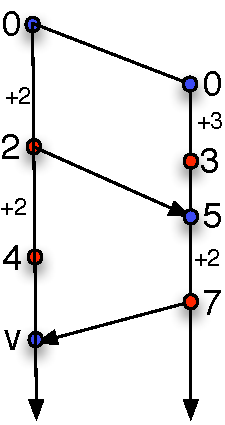
\includegraphics[scale=0.6]{Figures/merge-needs-lca}
\caption{This example of a grow-only counter illustrate why \C{merge}
needs a least common ancestor, and not just a common ancestor. Both 0
and 2 are common ancestors of 4 and 7, while 2 is their least common
ancestor (since $0 \preceq 2$). The result (v) of merging 4 and 7 is
11 (incorrect) if 0 is used as the common ancestor for merge, and 9
(correct, because 2+2+3+2 = 9) if 2 is used. }
\label{fig:merge-needs-lca}
\end{wrapfigure}
not be the case. With unrestrained branching and merging, there is no
bound on the number of LCAs a pair of versions can have.  For example,
in Fig.~\ref{fig:criss-cross-lcas}, the merge of 0 with 3 is preceded
by two ``criss-cross'' merges between their respective
branches\footnote{
  When discussing merges and LCAs, we often attribute the properties
  of latest versions on branches to the branches themselves.  For
  instance, when we say two branches merge, in fact their latest
  versions merge. Likewise, LCA of two branches means the LCA of their
  latest versions.
}
resulting in there being two LCAs (5 and 4) for 0 and 3. 
Multiple LCAs can occur even without criss-cross merges, as
demonstrated by Fig.~\ref{fig:external-lcas}. 
Concurrent versions with multiple LCAs do not lend themselves to
three-way merging. If such versions are latest on their respective
branches, they render the branches unmergeable (since  \C{lca} is no
longer a function) as demonstrated by examples in
Fig.~\ref{fig:many-lcas}. Note that for both the examples in
Fig.~\ref{fig:many-lcas}, no extension of the branching structure
can make the branches merge again. Thus the system is effectively
\emph{partitioned} permanently. This is clearly a problem. 

\begin{figure}[!t]
\centering
\subcaptionbox[] {\small
  In this example, 1 and 3 have two LCAs (3 and 4) a result of
  previous merges. The dotted circle denotes a virtual ancestor
  obtained by merging the two LCAs.
  \label{fig:criss-cross-lcas}
} [0.47\columnwidth] {
  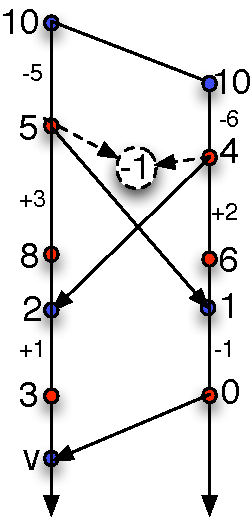
\includegraphics[scale=0.55]{Figures/2-LCAs}
}
\hfill
\subcaptionbox[] {\small
  In this example, versions $v_{13}$ and $v_{44}$ have two LCAs
  ($v_{22}$ and $v_{32}$)  despite there not being any previous merges
  between their respective branches.
  \label{fig:external-lcas}
} [0.47\columnwidth] {
  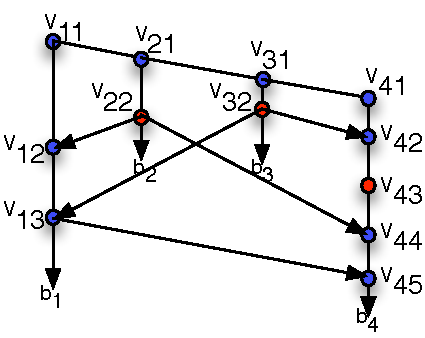
\includegraphics[scale=0.7]{Figures/2-external-LCAs}
}
\caption{Examples where two branches have more than one LCA, hence
cannot merge. }
\label{fig:many-lcas}
\end{figure}

The problem of multiple LCAs also arises in the context of source
control systems, which employ \emph{ad hoc} mechanisms to pave the way
for three-way merging.  GitHub~\cite{github}, for instance,
recursively merges LCAs to compute a virtual ancestor, which then
serves as the LCA for merging concurrent versions. This method is
demonstrated in the branching structure for a mergeable, replicated
counter as shown in Fig.~\ref{fig:criss-cross-lcas}, where LCAs 5 and
4 of 0 and 3 are merged (with their LCA being 10) to generate -1 as
the virtual LCA to merge 5 and 4. A major downside with this approach
is that it makes no guarantees on the relationship between the virtual
ancestor and its concurrent versions; the former may not even be a
legal ancestor of the latter as per the semantics of the data type.
For instance, suppose the integer type in
Fig.~\ref{fig:criss-cross-lcas} represents a bank account balance,
which is expected to disallows any activity on the account if the
balance is ever known to be less than zero.  From the perspective of
the library designer and its clients, there is no meaningful scenario
in which versions 3 and 0 can emerge from -1, since the only
transition allowed by the semantics from -1 is to itself.  Clearly,
\emph{ad hoc} mechanisms like this are error-prone and difficult to
apply in general.

Fortunately, unlike source control systems where branching structure
is entirely dictated by the user, \name abstracts away branching
structure from the programmer, and hence retains the ability to
manifest it in a way that it deems fit. In particular, \name solves
the problem of multiple LCAs by suitably constraining the branching
structure such that the problem never arises. The constraints are
imposed either implicitly, as a result of how operational semantics
defines an atomic step, or explicitly, by insisting that certain
conditions be met before merging a pair of versions
(\rulelabel{E-Pull-Wait}). Firstly, the operational semantics already
disables criss-cross merges since it only ever merges versions that
are latest on their respective branches. For instance, suppose
$v_{11}$ and $v_{21}$ are the latest versions on branches $b_1$ and
$b_2$, respectively. Merging $b_2$ into $b_1$ entails merging $v_{21}$
into $v_{11}$ to generate version $v_{12}$ on $b_1$.  Now, merging
$b_1$ into $b_2$ involves merging $v_{12}$, the latest version on
$b_1$, into $v_{21}$, but not $v_{11}$ into $v_{21}$, thus preempting
a criss-cross branching structure.

Secondly, we impose certain pre-conditions on the merging branches to
preempt the structure shown in Fig.~\ref{fig:external-lcas}. The
intuition is as follows: consider the branch $b_3$ at the instance of
merging $b_1$. Since it has already merged $b_2$, a version on $b_2$
($v_{21}$) could be a common ancestor for $b_3$ and some other branch
(call it $b$). Now, if $b_3$ merges $b_1$, same could be true of $b_3$
and $b_1$: a version on $b_1$ ($v_{11}$) could be a common ancestor
for $b_3$ and the other branch $v$. Since $v_{21}$ is also a common
ancestor for both the branches, and the ancestors are not ordered by
the ancestor relation, $b_3$ and $b$ end up with two LCAs. In
Fig.~\ref{fig:external-lcas}, the role of $b$ is played both by $b_1$
and $b_2$. We observe that this scenario can be prevented if, when
merging $b_1$, $b_3$ insists on an ancestor relation between the last
merged version ($v_{22}$ of the $b_2$), and the latest version of
$b_1$, the currently merging branch. We call the last merged version
the \emph{external locus} of the branch. By requiring that, for every
branch $b$, the external locii of $b$ at various points in time (i.e.,
external locus of every prefix of $b$) be totally ordered, and given
that the semantics already preempts criss-cross merges, we effectively
avoid the case of there ever being more than 2 LCAs for a pair of
branches. Thus, uniqueness of LCAs is thus guaranteed.

We now formalize the aforementioned intuitions via a series of
definitions, and theorems.

\begin{definition} [\bfseries Internal and External Ancestors]
Given a branch $b$ and a version $v\in b$, an internal ancestor of $v$
is an ancestor from the same branch $b$. An external ancestor of $v$
is an ancestor from a different branch $b'\neq b$. 
\end{definition}

\begin{definition} [\bfseries External Locus]
Given a branch $b$ and a version $v\in b$, external locus ($v_o$) of
$v$ is an external ancestor that is not an ancestor of any other
external ancestor of $v$. That is, $\under{H}{v_o \preceq v}$, and
there does not exist a $v_o' \not\in b$ such that $\under{H}{v_o'
\preceq v}$ and $\under{H}{v_o \preceq v_o'}$. 
\end{definition}

Note that internal ancestor relation ($\preceq_i$) is, by definition,
a total order. We later prove that the external ancestor relation
($\preceq_o$) is also a total order. Hence, for any given version $v$,
least internal and external ancestors, if exist, must be unique.  We
call the unique least internal ancestor as its \emph{internal locus},
and the unique least external ancestor version as its \emph{external
locus}. 

\begin{definition} [\bfseries Mergeability]
\label{def:mergeability}
Given a history $H$, a version $v_1$ and a version $v_2$ that is not
an ancestor of $v_1$ under $H$, $v_2$ is mergeable into $v_1$ (denoted
$\under{H}{v_2 \mbleto v_1}$) iff $v_1$'s external locus is an
ancestor of $v_2$.
\end{definition}

\begin{lemma} [\bfseries Unique External Locus]
Every version $v$ (except the \C{INIT} version) in the history $H$
generated by the rules in Fig.~\ref{fig:opsem} has a unique external
locus.
\end{lemma}

\begin{lemma} [\bfseries Unique LCA]
Every pair of branches in the history $H$ generated by the rules in
Fig.~\ref{fig:opsem} have a unique least common ancestor. 
\end{lemma}

\begin{lemma} [\bfseries Non-Monotonicity of Mergeability]
In a legal branching history $H$ produced by the operational
semantics, if two branches, $b_i$ and $b_j$ are not mergeable (as per
Def.~\ref{def:mergeability}), then there exist a series of merges
involving only the mergeable branches that can be performed on $H$ to
yeild a new history $H'$, where $b_i$ and $b_j$ are now mergeable.
\end{lemma}

\begin{theorem} [\bfseries Progress and Eventual Convergence] Given a
legal branching history $H$, and a program $p$, where every thread
expression in $p$ is a \C{pull}, there exist a series of reduction steps
that reduce $p; H$ to $p'; H'$, where every thread expression in $p$
is the same value $v$.
\end{theorem}


